\documentclass[conference]{IEEEtran}
\IEEEoverridecommandlockouts
% The preceding line is only needed to identify funding in the first footnote. If that is unneeded, please comment it out.
\usepackage{cite}
\usepackage{amsmath,amssymb,amsfonts}
\usepackage{graphicx}
\usepackage{textcomp}
\def\BibTeX{{\rm B\kern-.05em{\sc i\kern-.025em b}\kern-.08em
T\kern-.1667em\lower.7ex\hbox{E}\kern-.125emX}}
\begin{document}

    \title{THE3\\
    }

    \author{\IEEEauthorblockN{Esref Ozturk}
    \IEEEauthorblockA{\textit{CENG} \\
    \textit{METU}\\
    Ankara, Turkey \\
    esrefozturk93@gmail.com}
    }

    \maketitle


    \section{Introduction}
    This report includes the discussions about CENG499 Machine Learning THE3 Homework \\

    \section{Discussion}

    \subsection{Cluster Means}

    \begin{figure}[htbp]
        \centerline{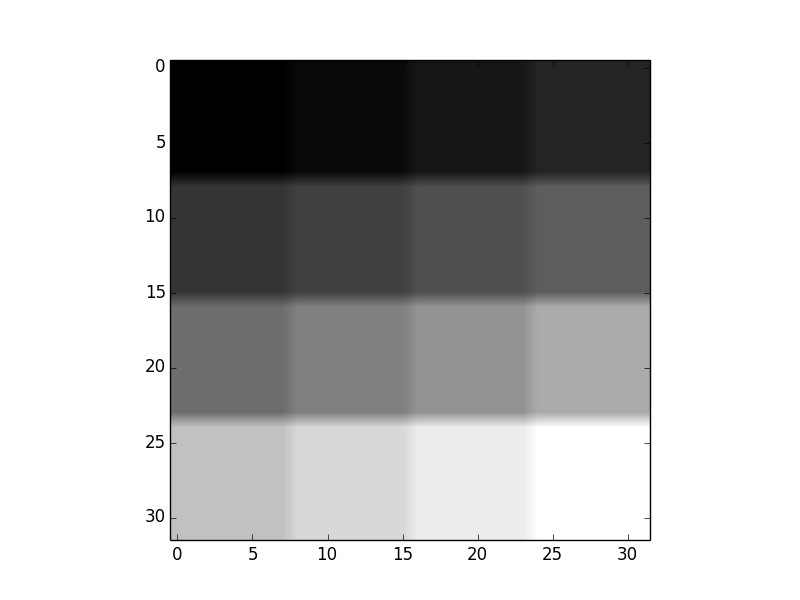
\includegraphics[width=0.5\textwidth]{16.png}}
        \caption{K=16}
        \label{k16}
    \end{figure}

    \begin{figure}[htbp]
        \centerline{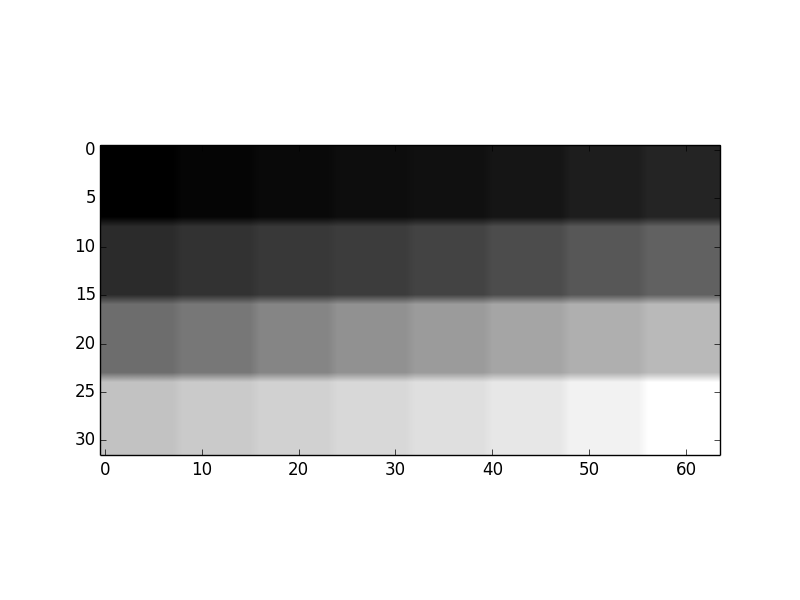
\includegraphics[width=0.5\textwidth]{32.png}}
        \caption{K=32}
        \label{k32}
    \end{figure}

    \begin{figure}[htbp]
        \centerline{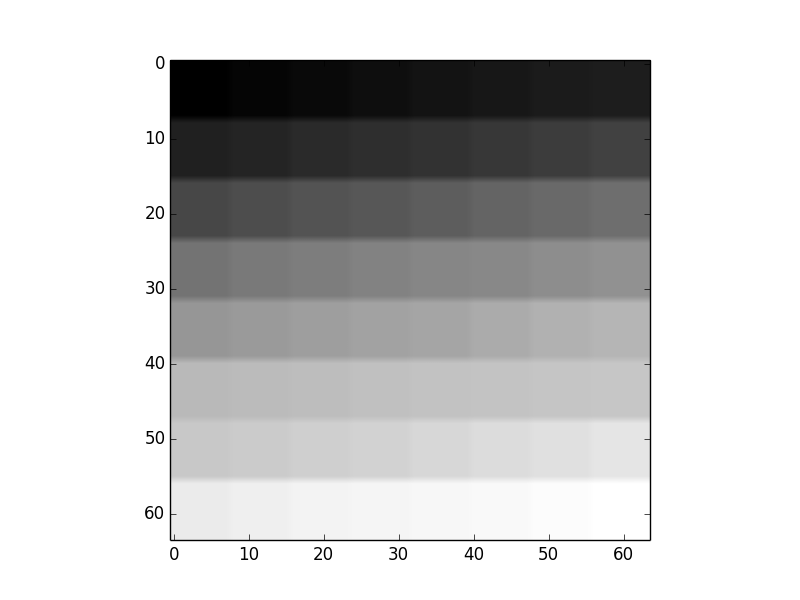
\includegraphics[width=0.5\textwidth]{64.png}}
        \caption{K=64}
        \label{k64}
    \end{figure}

    For every K, we have found K colors that are representing the dataset. If we divide dataset to K groups, we can represent each group with each color. As K increases, the max and min color is almost the same but transition is getting slow.

    \subsection{Principle Components}

    \begin{figure}[htbp]
        \centerline{\includegraphics[width=0.5\textwidth]{pca.png}}
        \caption{First 16 Principle Components}
        \label{pca}
    \end{figure}

    These are the simplest 16 images we can sum all 165 images up.


\end{document}
